\section{Front-End}\label{sec:5-front-end}
An important part of the UrbanSearch system is the part where the extracted and processed data are visualised and made accessible to the end user. Our goals were to provide the end users with a clear and easy to use interface. Extracted relations should therefore be visualised in such a way that the user can make sense of the information easily. Another desire that was expressed by our client, was the possibility to manipulate the displayed information, in a fast, easy and intuitive way. To keep the front-end flexible we decided to separate the front-end from the API. This way we can easily make changes to both systems while not having to worry about breaking either system.

\subsection{Technical Overview}
In this section we will discuss some of the main technical aspects of the UrbanSearch project. We will give an overview of and a motivation for our most important design choices.

\subsubsection{Modular Design}
Dealing with huge amounts of data and displaying this data in a way that makes this easy to understand for users is a challenging task. The complexity of handling the data and making it easy to manipulate by the end user means an increase in the complexity of our code. Besides this, the evolving desires of our client for viewing and manipulating the data lead us to using a modular implementation of the front-end.
Besides the fact that this approach increases readability, maintainability and extensibility it is also a best practice in the front-end realm\footnote{\url{https://developers.google.com/web/fundamentals/}}.\\
Modular development means writing self-contained elements of a web page, consisting of HTML, CSS and JavaScript. The components can be reused easily throughout the entire page and can be initialised with different sets of data to alter their appearance or functionality.\\
We also used the concept of container and presentational components\footnote{\url{https://medium.com/@dan_abramov/smart-and-dumb-components-7ca2f9a7c7d0}}. The idea behind this is that container components are concerned with the application logic. Presentational components on the other hand, are concerned with how elements looks, e.g. the styling and appearance of elements.\\
We believe that this approach will result in readable, maintainable and extensible code, which will allow for future proof code.
\subsubsection{NodeJS}
We chose NodeJS as the backbone of our front-end server. The fact that NodeJS is easy to setup and has a lot of modules that are quickly accessible through NPM\footnote{\url{https://www.npmjs.com}} was one of the main reasons for selecting NodeJS. Having a server running in a matter of minutes is a big advantage for a short project.\\
\replace{Another interesting feature of NodeJS}{not a feature!} are tools like Webpack and Gulp. Webpack\footnote{\url{https://webpack.js.org/concepts/}} is a module bundler for NodeJS that provides us with the ideal infrastructure for modular development. It allows us to bundle JavaScript code in different files, containing only the required code for a specific page. Gulp\footnote{\url{http://gulpjs.com/}} is a task runner for NodeJS that allows for tasks such as compiling HTML templates that can later be used in the front-end. Another example of a Gulp task is bundling the CSS of all the modules to one file.
\subsubsection{ExpressJS}

community standard
easy setup
easy to extend with custom middleware

\subsection{Interfaces}
In this section 
\subsubsection{Interactive Map}
\todo{mention threshold for relation total somewhere, including excel graph}
The main part of the front-end is the interactive map. The extracted data gets visualised on a (almost) full-screen Google Maps map. On the map we place markers which represent cities and we draw poly-lines which represent relations between the cities.

\begin{figure}[H]
\centering
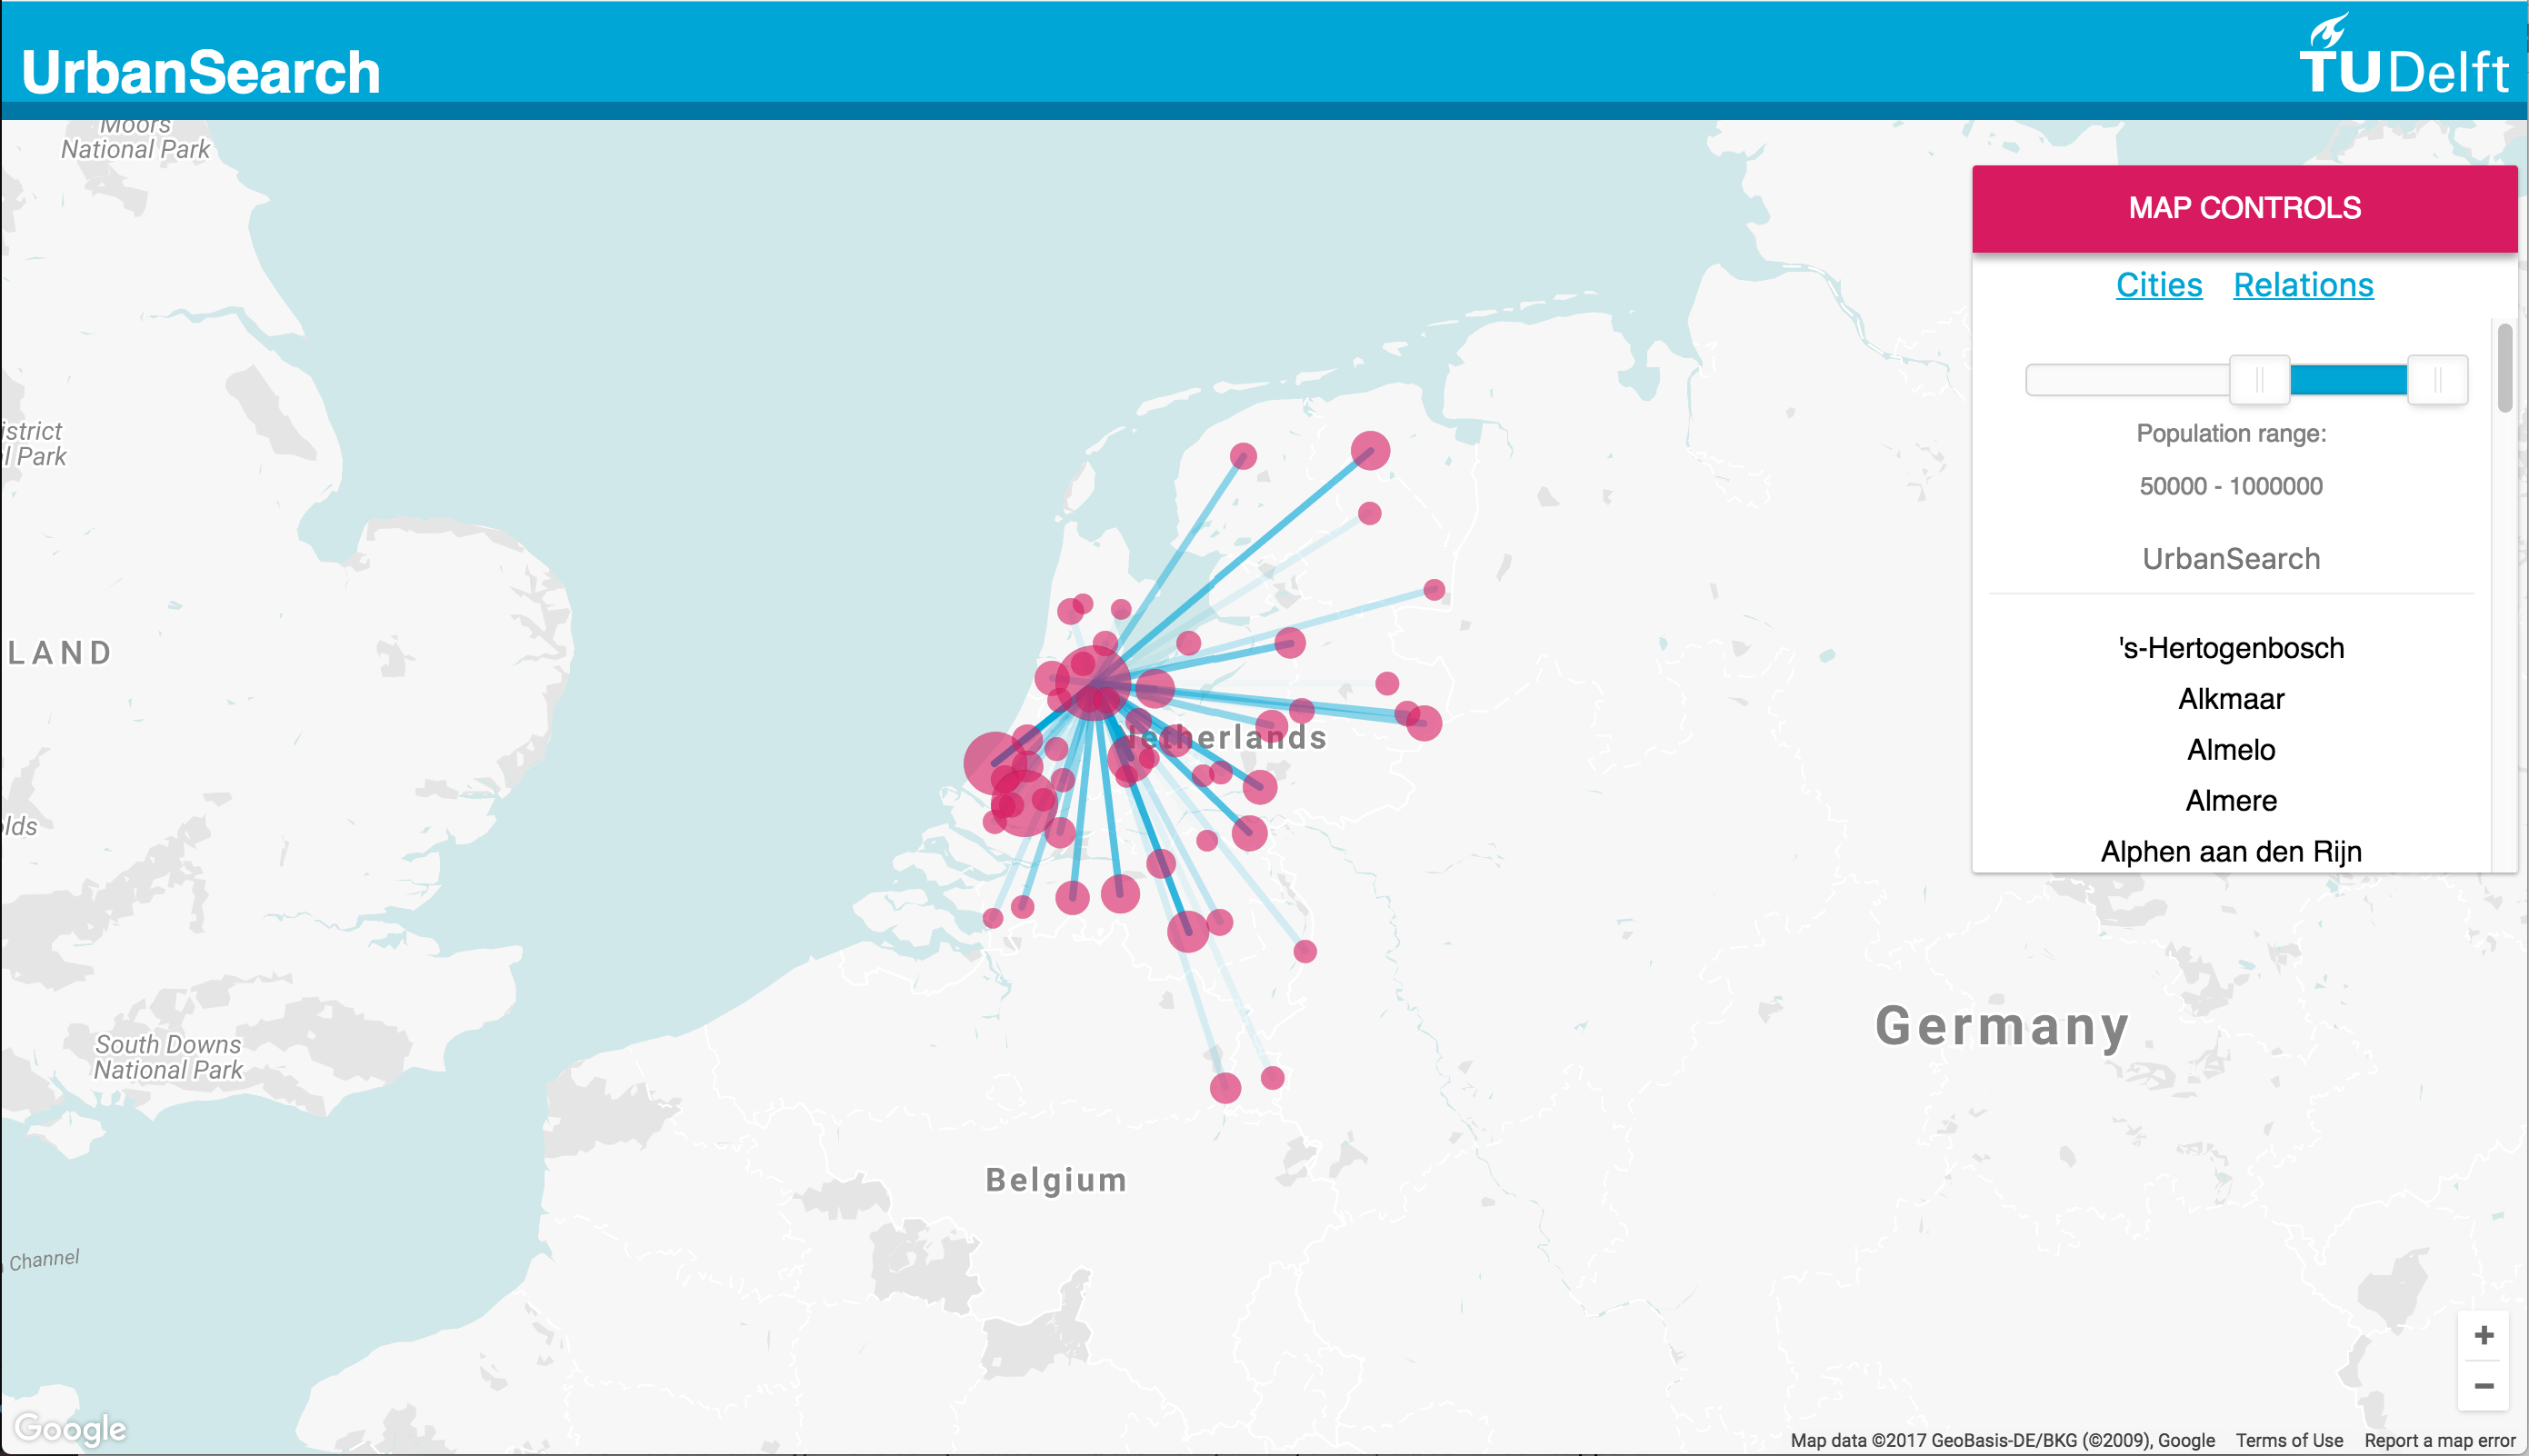
\includegraphics[width=0.8\textwidth]{frontend-map}
\caption{View on page-load of the interactive map}
\label{fig:frontend-map}
\end{figure}

On the right side of the interface a "Map Controls" card is always shown. This card lets users manipulate the data shown on the map. Since we have two main entities of interest (cities and relations) that are shown on the map, the controls offer an intuitive way to control these.\\

\begin{figure}[H]
\centering
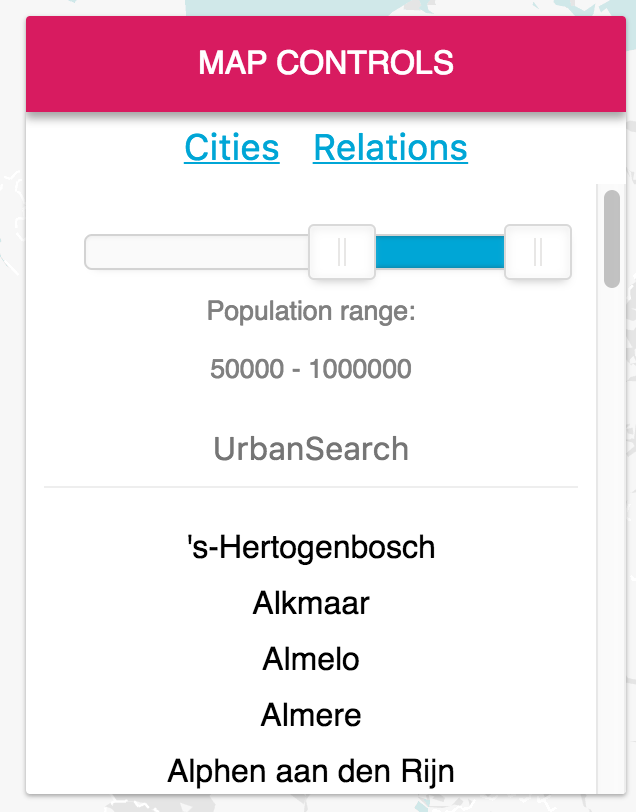
\includegraphics[width=0.5\textwidth]{frontend-mc}
\caption{Map Controls for the interactive map - Cities}
\label{fig:frontend-mc}
\end{figure}

Cities are indicated by the circles on the map. The circles have an diameter that is calculated based on the population size of the city. Figure \ref{fig:frontend-mc} shows the controls for the city entities. The slider shown in the upper part of the card allows to filter cities based on population. All cities that fall in the range of the slider are shown, all other are not visible. Besides displaying and hiding cities based on population size, users can also toggle visibility of cities by clicking on the cities displayed in the list below the slider.\\
Relations are shown as poly-lines on the map. The total strength of the relation (which will be discussed below) is used to set an opacity for the relation, like show in figure \ref{fig:frontend-rel-strength}. A low opacity indicates an strong total strength of the relation and vice versa.

\begin{figure}[H]
\centering
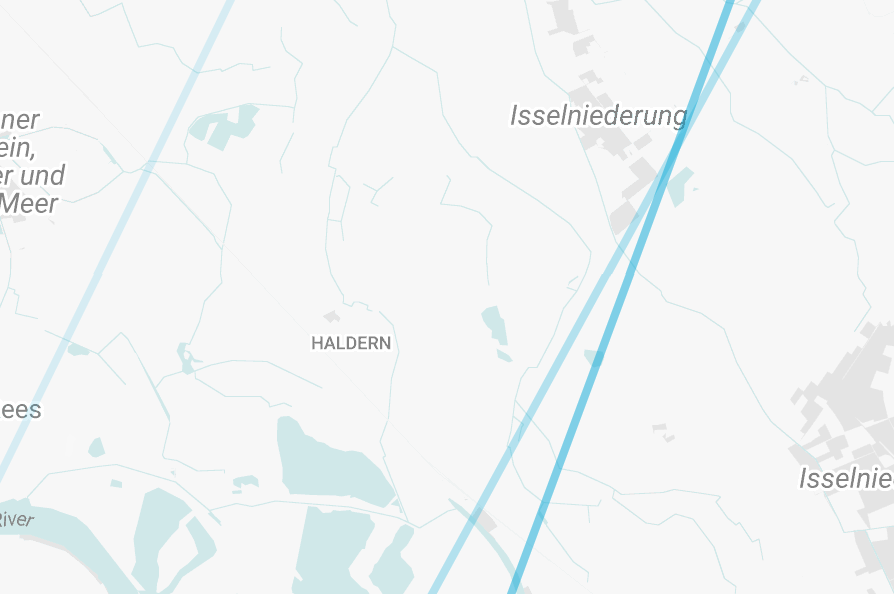
\includegraphics[width=0.7\textwidth]{frontend-rel-strength}
\caption{Different relation strengths are shown by adjusting opacity}
\label{fig:frontend-rel-strength}
\end{figure}

The relations controls are shown in figure \ref{fig:frontend-mc-rel}. Here the user can select which relations are considered when calculating the total relation strengths. This is done by clicking the check-boxes next to the relation names. The sliders provide a way to filter the relations based on the total relation strength for the category belonging to the slider.\\

\begin{figure}[H]
\centering
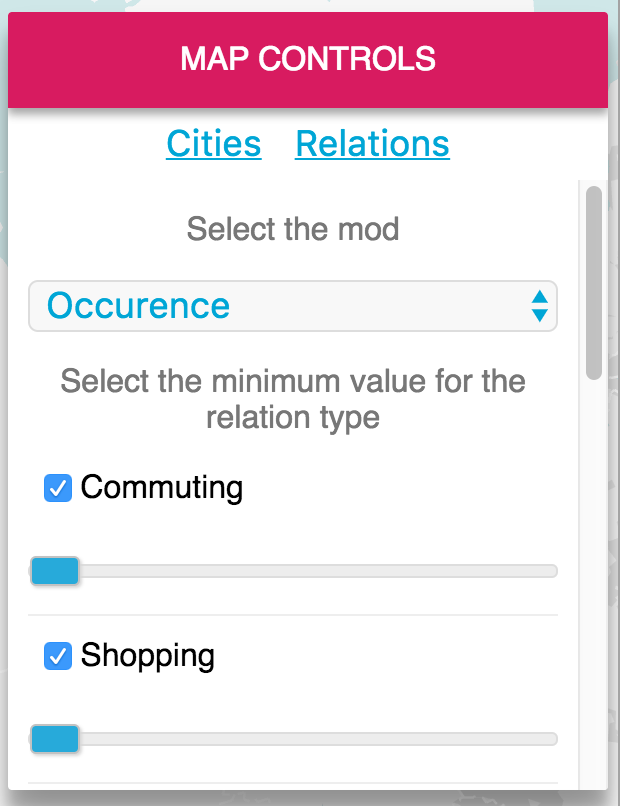
\includegraphics[width=0.5\textwidth]{frontend-mc-rel}
\caption{Map Controls for the interactive map - Relations}
\label{fig:frontend-mc-rel}
\end{figure}

The drop-down shown in the relations control interface provides a way to scale the relation totals. Lets say for example that we do not want the absolute count of occurrences as a measure for total relation strength but that we want it scaled relative to the population size of two cities. This can be done by selecting the right option in the drop-down.\\
All of these features are meant to provide the user with means for constructing a visualisation that uncovers patterns which are not (easily) seen when looking at raw data.
\subsubsection{Document Classification}
The document classification interface is meant as an easy way of extending our data-set which is used to train and test our classifier. The interface loads documents that we have deemed relevant while analysing the available CommonCrawl pages. The user can select one or multiple categories which the user feels best relate to the document. If the user finds the document to be irrelevant the document can be discarded. An example of the interface with a document belonging in the "collaboration" category is shown in figure \ref{fig:frontend-label}).
\begin{figure}[H]
\centering
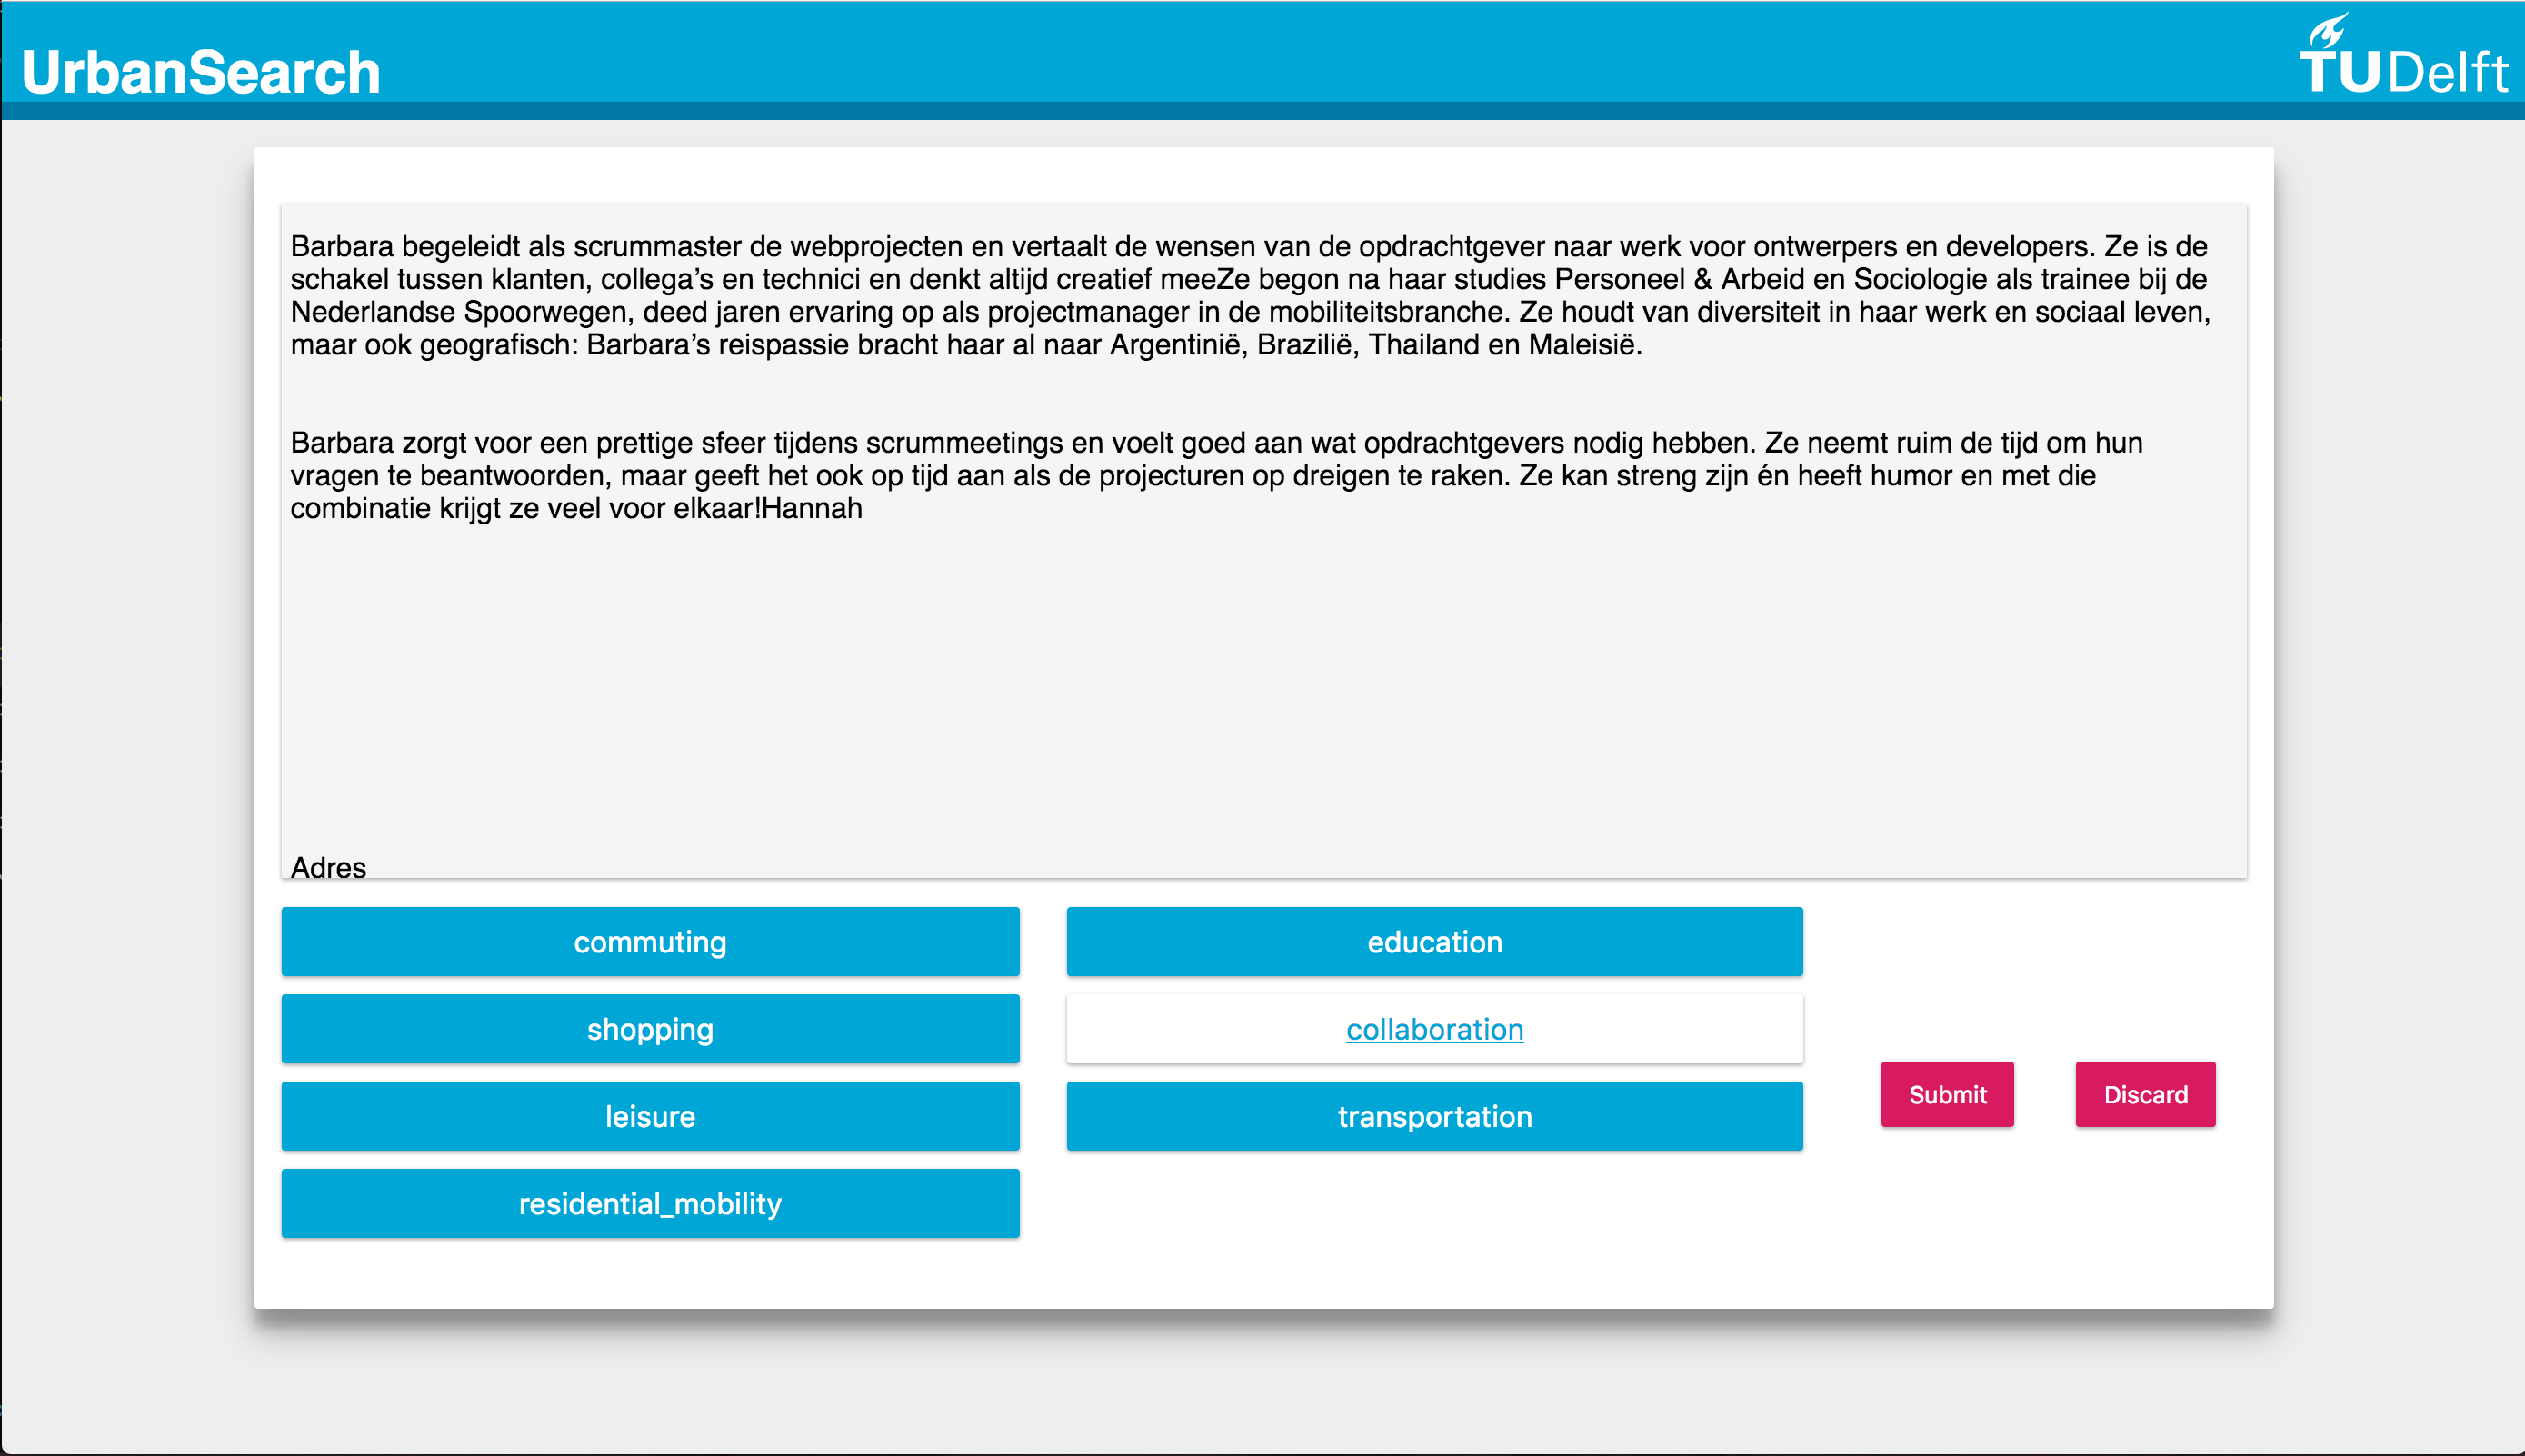
\includegraphics[width=0.8\textwidth]{labelling_interface}
\caption{The labelling interface}
\label{fig:frontend-label}
\end{figure}

\subsubsection{System Settings}

Both the back end and the front end of the UrbanSearch system share and depend on some default settings. To keep the system configurable, even for an user that is not a developer, we have implemented a system settings interface (figure \ref{fig:frontend-ss}). The interface can be extended with more settings as the user likes. This is achieved by the loose coupling of the front end and the API that was mentioned before.


\begin{figure}[H]
\centering
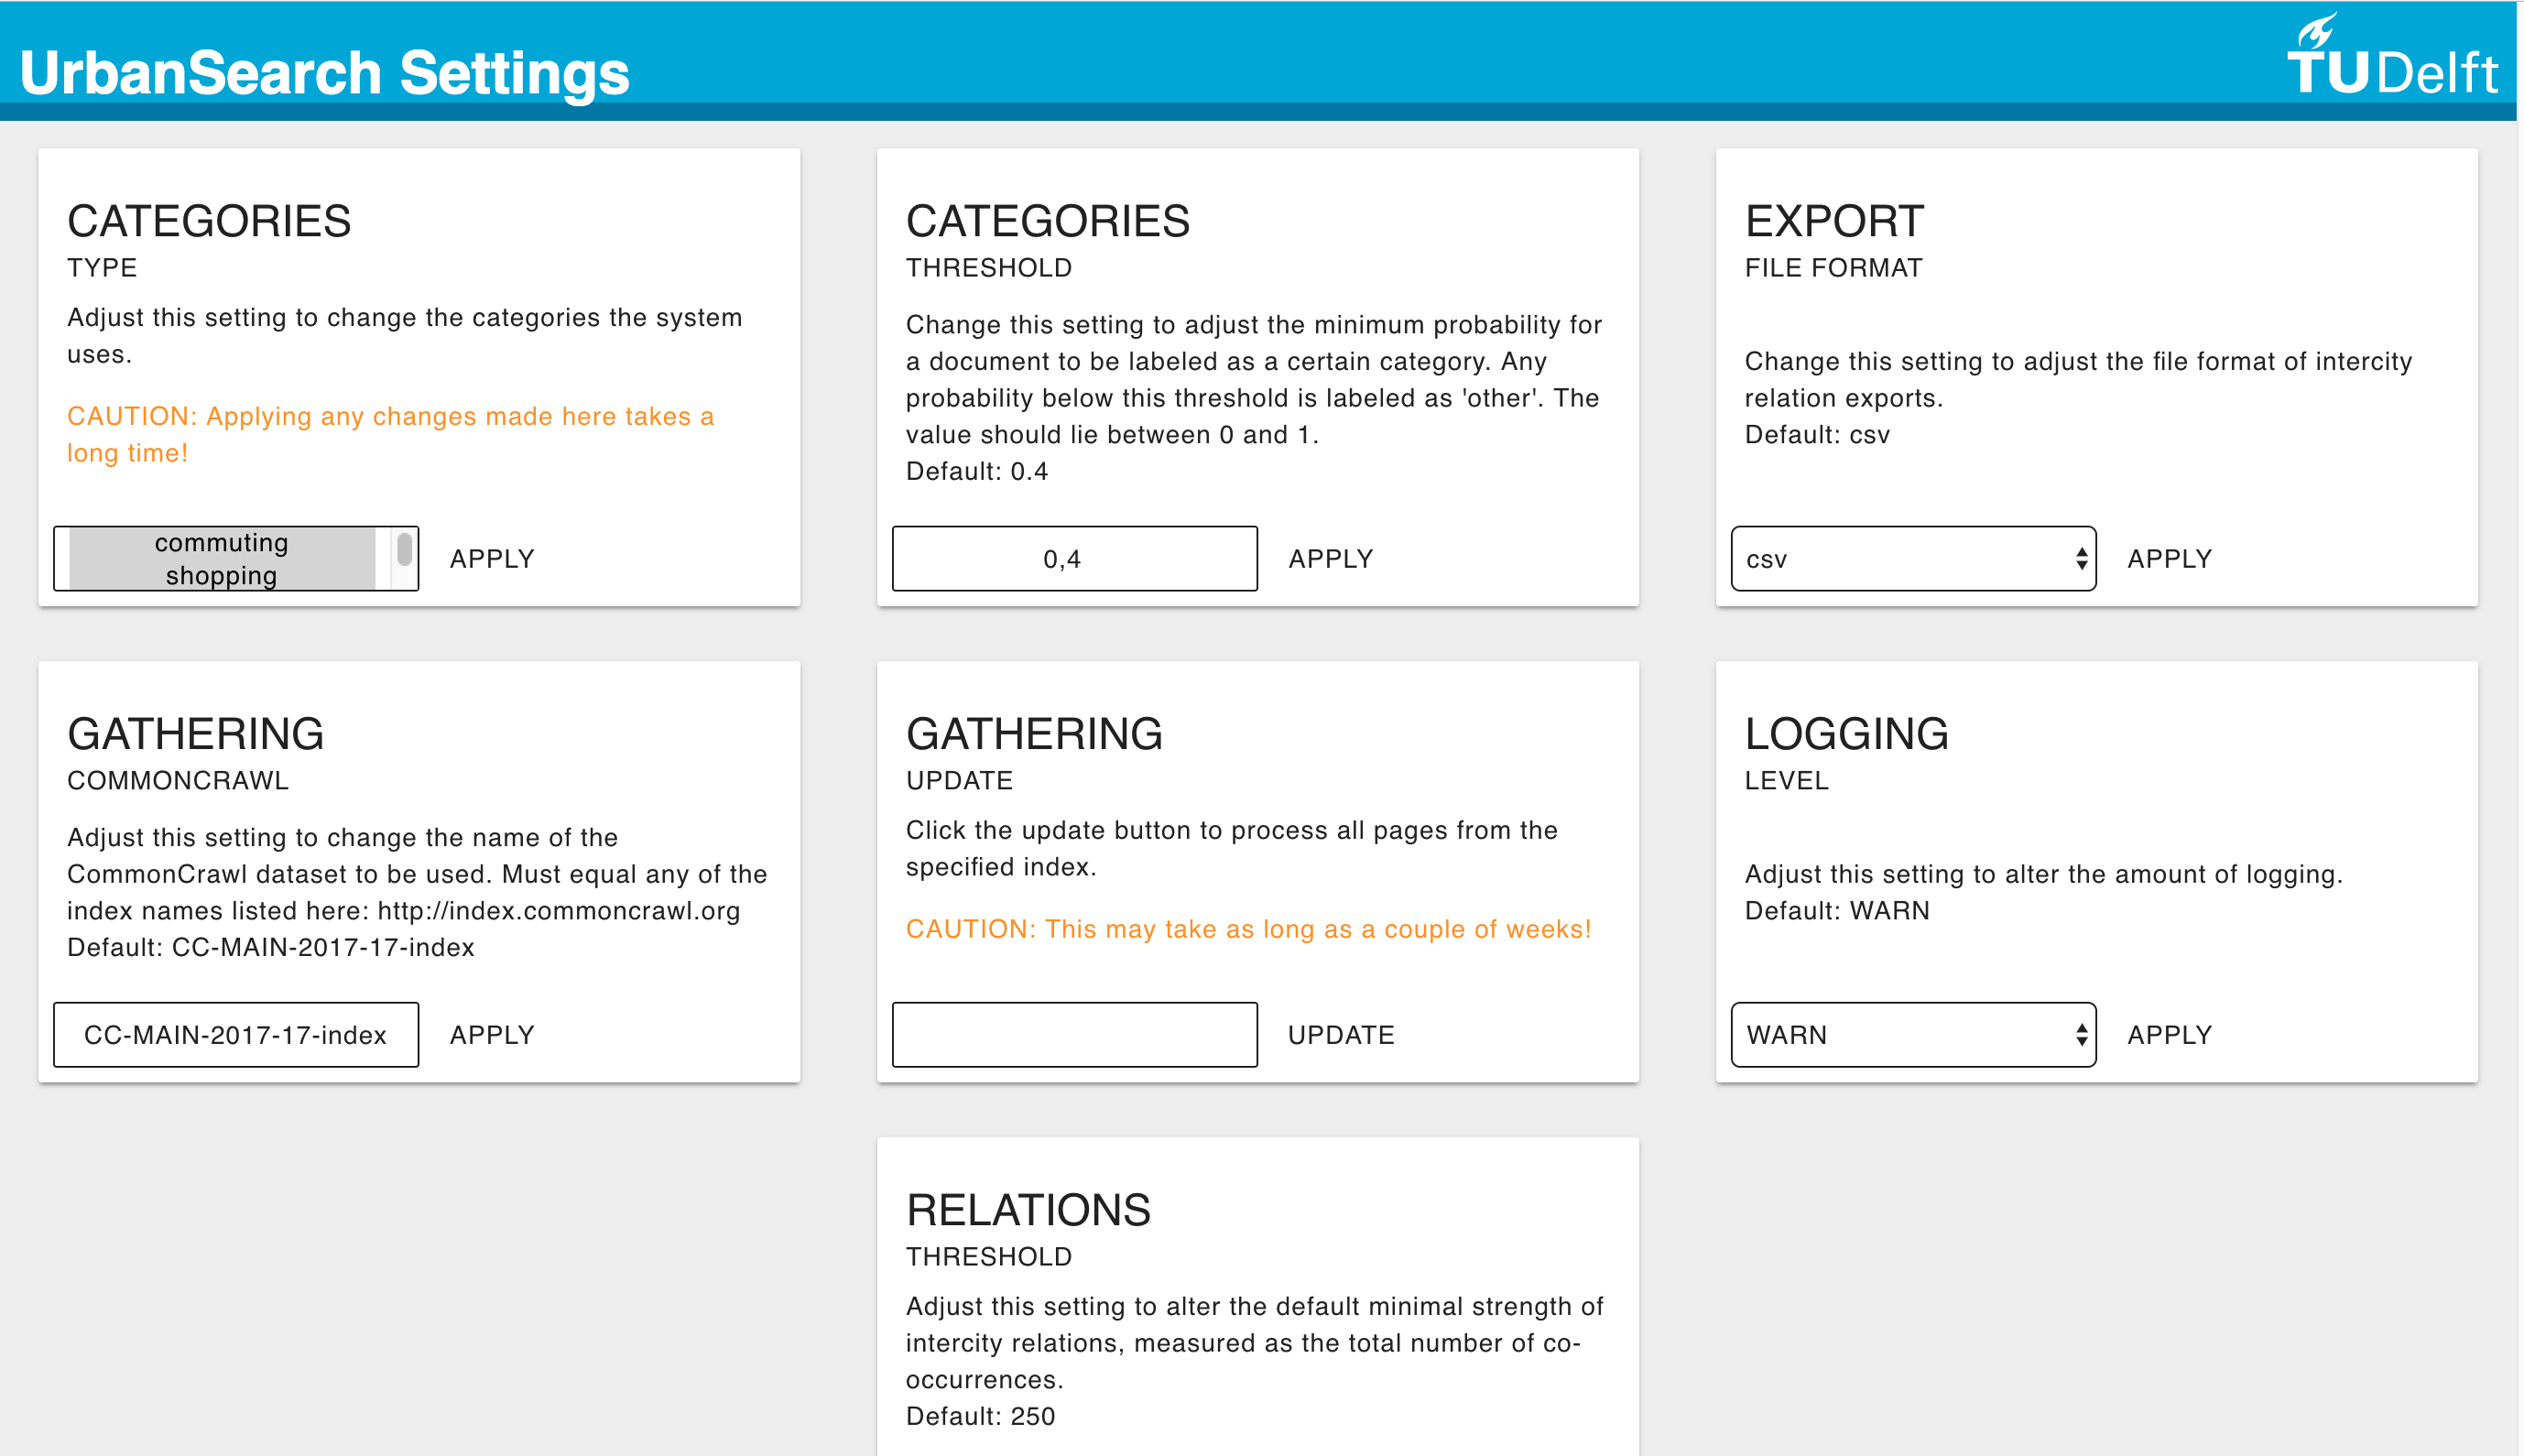
\includegraphics[width=0.8\textwidth]{frontend-ss}
\caption{The systems settings interface}
\label{fig:frontend-ss}
\end{figure}